\section{Auswertung}
\label{Auswertung}
\subsection{Bestimmung des Sättigungsstroms}
\label{Auswertung_a}

Die Daten der Messung vom Strom $I$ in Abhängigkeit von der Spannung $U$ zwischen Anode und Kathode befinden sich in Tabelle \ref{tab:a1} \& \ref{tab:a2}. Diese Werte sind in der Abbildung \ref{fig:Kennlinie} grafisch abgebildet.

\begin{table} [H]
	\centering
	\caption{Messdaten der Hochvakuumdiode ($I_1$ bis $I_4$).}
	\label{tab:a1}
	\sisetup{table-format=4.2}
	\begin{tabular}{S[table-format=4.2]|cccc}
		\toprule
		{$\frac{U}{V}$}&{$\frac{I_1}{mA}$}&{$\frac{I_2}{mA}$}&{$\frac{I_3}{mA}$}&{$\frac{I_4}{mA}$} \\
		\midrule
		10 &0.022&0.029&0.034&0.036\\
		20 &0.048&0.067&0.078&0.087\\
		39 &0.079&0.109&0.134&0.146\\
		40 &0.105&0.155&0.191&0.216\\
		50 &0.118&0.202&0.252&0.288\\
		60 &0.130&0.248&0.323&0.371\\
		70 &0.138&0.281&0.385&0.453\\
		80 &0.145&0.305&0.444&0.527\\
		90 &0.148&0.310&0.511&0.625\\
		100 &0.150&0.329&0.560&0.716\\
		110 &0.153&0.340&0.615&0.801\\
		120 &0.155&0.348&0.661&0.884\\
		130 &0.156&0.354&0.689&0.955\\
		140 &0.158&0.357&0.716&1.035\\
		150 &0.159&0.361&0.739&1.100\\
		160 &0.160&0.362&0.753&1.165\\
		170 &0.161&0.363&0.763&1.217\\
		180 &0.161&0.365&0.773&1.268\\
		190 &0.162&0.367&0.780&1.316\\
		200 &0.162&0.369&0.788&1.353\\
		\bottomrule 
	\end{tabular}
\end{table} 

\begin{table} [H]
	\centering
	\caption{Messdaten der Hochvakuumdiode ($I_5$, maximale Heizleistung).}
	\label{tab:a2}
	\sisetup{table-format=4.2}
	\begin{tabular}{S[table-format=4.2]|c}
		\toprule
		{$\frac{U}{V}$}&{$\frac{I_5}{mA}$} \\
		\midrule
		5 &0.015\\
		10 &0.032\\
		15 &0.055\\
		20 &0.080\\
		25 &0.109\\
		30 &0.145\\
		35 &0.181\\
		40 &0.220\\
		45 &0.265\\
		50 &0.303\\
		55 &0.352\\
		60 &0.417\\
		65 &0.466\\
		70 &0.514\\
		75 &0.578\\
		85 &0.683\\
		95 &0.801\\
		105 &0.950\\
		115 &1.096\\
		125 &1.227\\
		135 &1.363\\
		145 &1.501\\
		155 &1.631\\
		165 &1.773\\
		175 &1.910\\
		180 &1.980\\
		185 &2.060\\
		190 &2.130\\
		195 &2.210\\
		200 &2.280\\
		205 &2.350\\
		210 &2.420\\
		215 &2.500\\
		220 &2.560\\
		225 &2.640\\
		230 &2.720\\
		235 &2.790\\
		240 &2.860\\
		245 &2.930\\
		250 &3.000\\
		\bottomrule 
	\end{tabular}
\end{table} 

\begin{figure}[H]
    \centering
    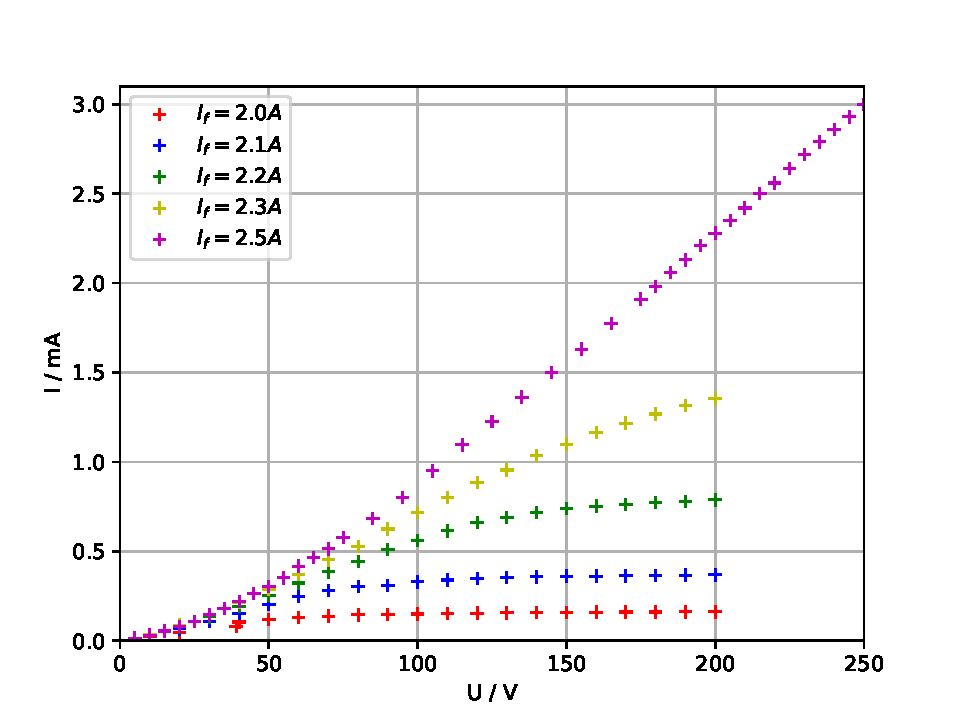
\includegraphics[scale=0.7]{Auswertung/Kennlinien.pdf}
    \caption{Kennlinie der Hochvakuumdiode.}
    \label{fig:Kennlinie}
\end{figure}

Aus diesen Kennlinien lässt sich der Sättigungsstrom $I_\text{S}$ ablesen. Er ist an der Abflachung der Kennlinie erkennbar. Es wird nicht der letzte Wert, sondern der Wert, bei dem keine Steigung mehr sichtbar ist, als Sättigungsstrom-wert verwendet. Sofern keine Abflachung erkennbar ist, wird der letzte gemessene Wert verwendet. Somit ergeben sich für die verschiedenen Heizströme $I_\text{f}$ folgende Sättigungsströme. Zu beachten ist jedoch, dass für den maximalen Heizstrom \\*$I_\text{f} = 2,5 \text{A}$ keine Sättigung zu erreichen war und somit lediglich der höchste gemessene Wert angegeben wird.
\begin{gather*}
	I_\text{S1} = 0,162 \text{mA} \\
	I_\text{S2} = 0,368 \text{mA} \\
	I_\text{S3} = 0,785 \text{mA} \\
	I_\text{S4} = 1,353 \text{mA} \\
	I_\text{S5} = 3,000 \text{mA}
\end{gather*}

\subsection{Untersuchung des Langmuir-Schottkyschen Gesetzes}
Aus den Messdaten aus Tabelle \ref{tab:a2} wird nun der Exponent der Strom-Spannungs-Beziehung bestimmt:
\begin{equation}
\label{Strom-Spannung}
	I = k \cdot U^{q}.
\end{equation}
Die Messdaten sind in Abbildung \ref{fig:b} doppelt logarithmisch dargestellt.
Mithilfe einer linearen Regression, welche ebenfalls in Abbildung \ref{fig:b} abgebildet ist, über curve-fit  von scipy.optimize und 
\begin{equation*}
	\text{ln}\left(\frac{I}{A}\right) = q \cdot \text{ln} \left(\frac{U}{V}\right) + \text{ln}\left(\frac{k}{A V^{-1}}\right)
\end{equation*}
ergeben sich somit folgende Werte:
\begin{gather*}
	q = \num{1.4163 \pm 6.6587}{10^{-5}} \\
	ln\left(\frac{k}{A V^{-1}}\right) = \num{-6.6868 \pm 0.0014}
\end{gather*}
\begin{figure}[H]
    \centering
    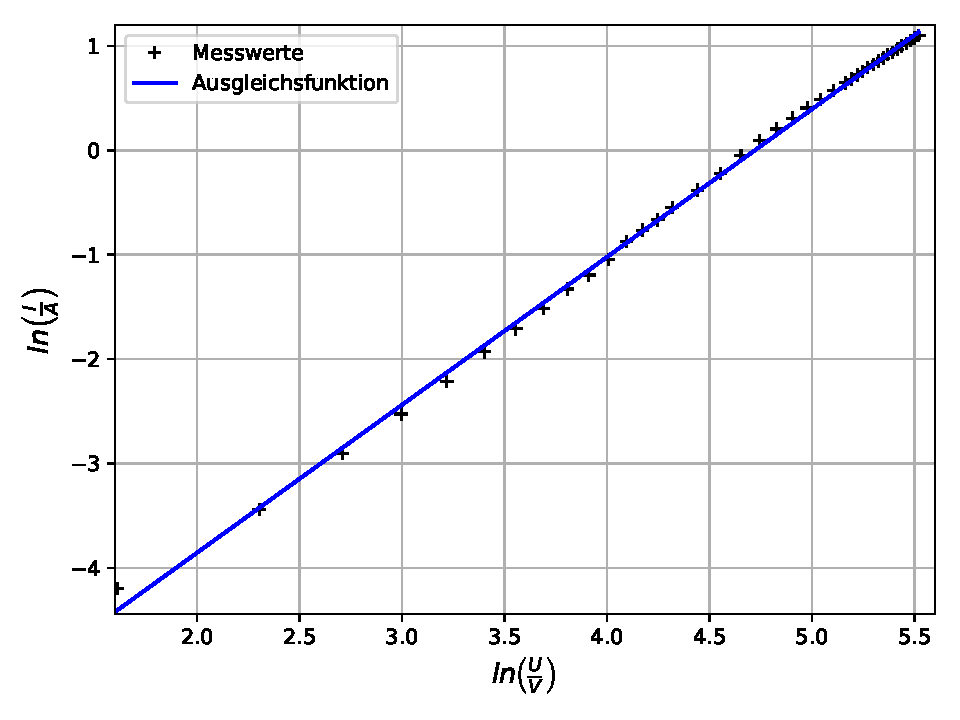
\includegraphics[scale=0.7]{Auswertung/b.pdf}
    \caption{Diodenkennlinie im Raumladungsgebiet bei $I_\text{H} = 2.5 \text{A}$.}
    \label{fig:b}
\end{figure}

Das Langmuir-Schottkysche Gesetz besagt für $q$ einen Wert von
\begin{equation*}
	q_{\text{theo}} = \frac{3}{2} \qquad [1].
\end{equation*}

Somit besteht eine Abweichung von 
\begin{equation*}
	\increment q = \frac{|q_{\text{theo}} - \bar{q}|}{q_{\text{theo}}} = 5,9\%.
\end{equation*}

\subsection{Anlaufstromgebiet \& Kathodentemperatur}

In Tabelle \ref{tab:c} ist der gemessene Diodenstrom $I$ bei angelegter Gegenspannung $U$ notiert. Das verwendete Amperemeter hat jedoch einen Innenwiderstand von 
\begin{equation*}
	R_{\text{i}} = 1 \text{M\Omega}
\end{equation*}
und kann daher nicht vernachlässigt werden. Somit ist in Tabelle \ref{tab:c} zusätzlich die korrigierte Gegenspannung $U_\text{c}$ aufgetragen. Diese wird durch
\begin{equation*}
	U_\text{c} = U + I \cdot R_\text{i}
\end{equation*}
berechnet.
\\
In Abbildung \ref{fig:Anlauf_Mess} sind die korrigierte Spannung $U_\text{c}$ und der Diodenstrom $I$ aufgetragen. 
Es gilt
\begin{equation*}
	I = C \cdot exp\left(\frac{e_0 U_\text{c}}{k_\text{b} T}\right).
\end{equation*}
Aus diesem Grund werden die Daten in Abbildung \ref{fig:Anlauf_Regress} halb-logarithmisch dargestellt und eine lineare Regression mit
\begin{equation*}
	\text{ln}\left(\frac{I}{A}\right) = \frac{e_0}{k_\text{b}T} \cdot U + \text{ln}(C) = m \cdot U + b
\end{equation*}
durchgeführt. \\
Aus dem Fit ergibt sich für die Steigung $m$
\begin{equation*}
	m = \num{4.812 \pm 0.005}.
\end{equation*}
Da $m = \frac{e_0}{k_\text{b}T}$, ergibt sich für die Kathodentemperatur $T$ der Wert
\begin{equation*}
	T = \SI{2411.1 \pm 2.5}{\kelvin}.
\end{equation*}

\begin{figure}[H]
    \centering
    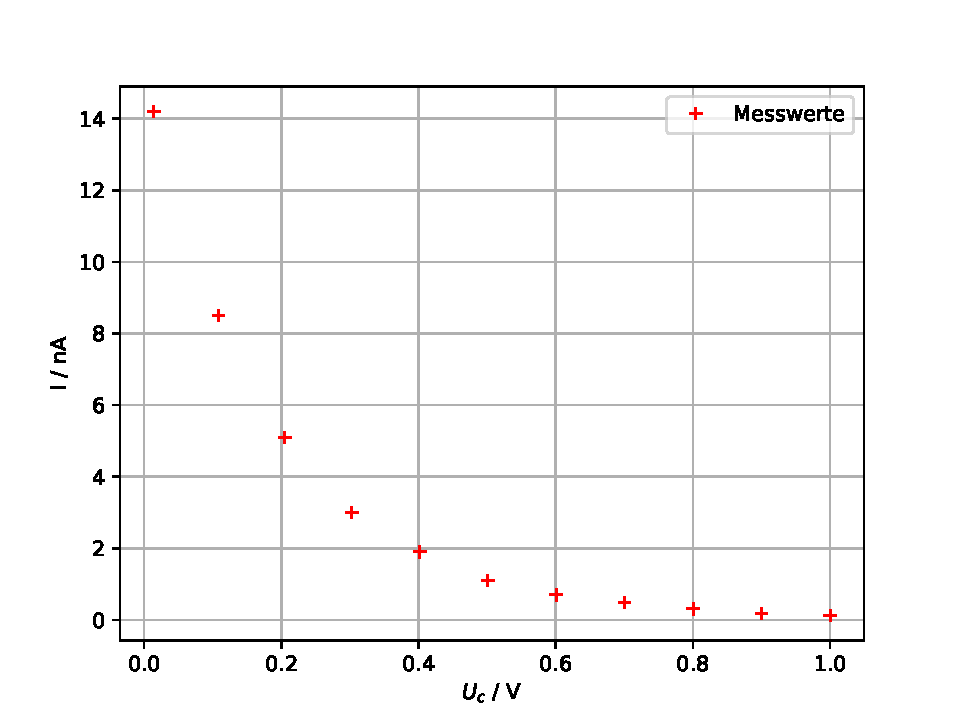
\includegraphics[scale=0.7]{Auswertung/c_Messwerte.pdf}
    \caption{Messwerte des Anlaufstromgebiets.}
    \label{fig:Anlauf_Mess}
\end{figure}
\begin{figure}[H]
    \centering
    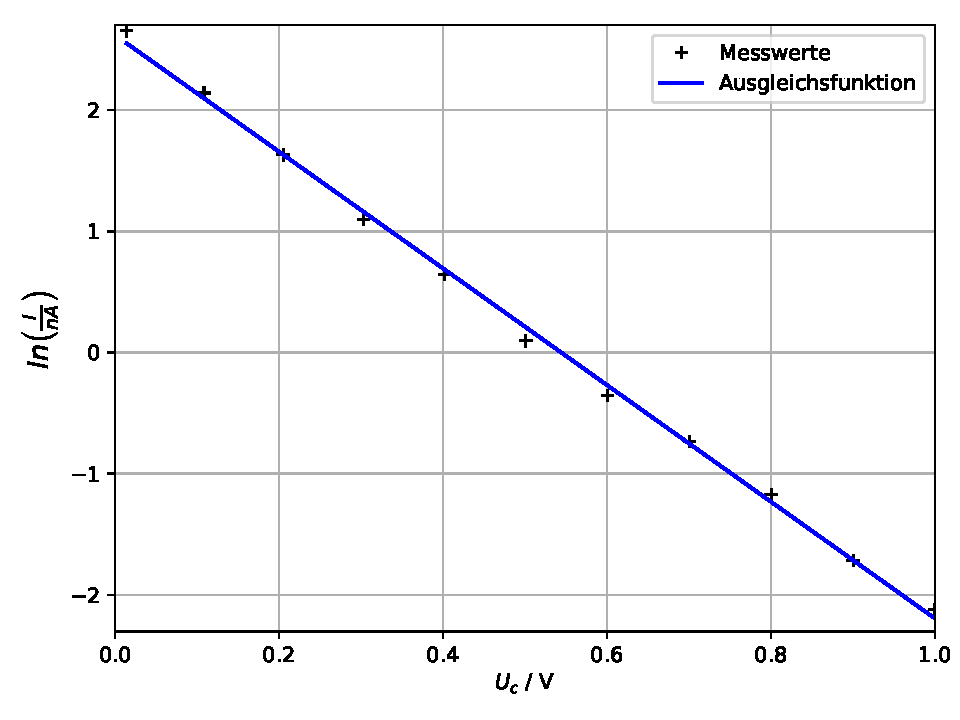
\includegraphics[scale=0.7]{Auswertung/c_Regression.pdf}
    \caption{Regression der Messwerte des Anlaufstromgebiets.}
    \label{fig:Anlauf_Regress}
\end{figure}

\begin{table} [H]
	\centering
	\caption{Strom bei (korrigierter) Gegenspannung im Anlaufstromgebiet und bei maximaler Heizleistung.}
	\label{tab:c}
	\sisetup{table-format=4.2}
	\begin{tabular}{S[table-format=4.2]ccc}
		\toprule
		{$\frac{U}{V}$}&{$\frac{U_{\text{c}}}{V}$}&{$\frac{I}{mA}$} \\
		\midrule
		0.0 &0.0142 &14.20\\
		0.1 &0.1085 &8.50\\
		0.2 &0.2051 &5.10\\
		0.3 &0.3030 &3.00\\
		0.4 &0.4019 &1.90\\
		0.5 &0.5011 &1.10\\
		0.6 &0.6007 &0.70\\
		0.7 &0.7005 &0.48\\
		0.8 &0.8003 &0.31\\
		0.9 &0.9002 &0.18\\
		1.0 &1.0001 &0.12\\
		\bottomrule 
	\end{tabular}
\end{table}	
	
\subsection{Kathodentemperaturen bei verschiedenen Heizleistungen}
Nun werden die Kathodentemperaturen bei den unterschiedlichen Heizleistungen aus Tabelle \ref{tab:a1} und \ref{tab:a2} bestimmt.
Dazu wird die Leistungsbilanz der Kathode verwendet
\begin{equation*}
	N_\text{zu} = N_\text{Str} + N_\text{WL},
\end{equation*}
wobei $N_\text{zu}$ die zugeführte Leistung, $N_\text{Str}$ die Strahlungsleistung und $N_\text{WL}$ die Wärmeleitung ist.
Die Wärmestrahlung $N_\text{Str}$ ist durch das Stefan-Boltzmannsche Gesetz definiert als
\begin{equation*}
	N_\text{Str} = A\eta\sigma T^4 .
\end{equation*}
Die Fläche der Kathode beträgt
\begin{equation*}
	A = \SI{0.32}{\square\centi\metre},
\end{equation*}
und der Absorptionsgrad 
\begin{equation*}
	\eta = 0,25   [1].
\end{equation*}
Somit ergibt sich für die Kathodentemperatur, bei einer Wärmeleitung von $N_\text{WL} = 1 \text{W}$:
\begin{equation*}
	T = \sqrt[4]{\frac{U_\text{H}I_\text{H} -1 \text{W}}{A\eta\sigma}} .
\end{equation*}
Hierbei ist 
\begin{equation*}
	\sigma = 5,6704 \cdot  10^{-8} \frac{\text{W}}{\text{m}^2\text{K}^4} .
\end{equation*}
$I_\text{H}$ und $U_\text{H}$ sind Heizstrom und Heizspannung. 
Die verwendeten Messdaten und Ergebnisse sind in der Tabelle \ref{tab:Temp} aufgetragen.

\begin{table} [H]
	\centering
	\caption{Berechnung der Kathodentemperatur.}
	\label{tab:Temp}
	\sisetup{table-format=4.2}
	\begin{tabular}{S[table-format=4.2]ccc}
		\toprule
		{$\frac{I_\text{H}}{A}$}&{$\frac{U_\text{H}}{V}$}&{$\frac{T}{K}$} \\
		\midrule
		2.0&4.0&1399.7\\
		2.1&4.5&1467.1\\
		2.2&4.8&1513.1\\
		2.3&5.0&1549.0\\
		2.5&6.0&1664.5\\
		\bottomrule 
	\end{tabular}
\end{table}

\subsection{Austrittsarbeit von Wolfram}
Mithilfe der Richardson-Gleichung \ref{eqn:rich} kann die Austrittsarbeit $W_\text{A}$ des Kathodenmaterials berechnet werden. Hierzu werden die zuvor bestimmten Werte des Sättigungsstroms $I_\text{S}$ und der Kathodentemperaturen $T$ verwendet. \\
Über die Gleichung
\begin{equation*}
	W_\text{A} = -\text{log}\left(\frac{I_\text{S}h^3}{e_0m_0k_\text{b}^2T^2}\right) \cdot k_\text{b}T
\end{equation*}
wird nun die Austrittsarbeit für Wolfram bestimmt. Die Ergebnisse sind in Tabelle \ref{tab:Austritt} aufgetragen.
\begin{table} [H]
	\centering
	\caption{Austrittsarbeit von Wolfram.}
	\label{tab:Austritt}
	\sisetup{table-format=4.2}
	\begin{tabular}{S[table-format=4.2]ccc}
		\toprule
		{$\frac{I_\text{S}}{mA}$}&{$\frac{T}{K}$}&{$\frac{W_\text{A}}{eV}$} \\
		\midrule
		0.161&1399.7&4.18\\
		0.368&1467.1&4.29\\
		0.781&1513.1&4.34\\
		1.353&1549.0&4.37\\
		3.000&1664.5&4.61\\
		\bottomrule 
	\end{tabular}
\end{table}
Daraus ergibt sich für den Mittelwert:
\begin{equation*}
	W_\text{A} = \num{4.36 \pm 0.07} \text{eV}
\end{equation*}
Der theoretische Wert für Wolfram beträgt
\begin{equation*}
	W_\text{A} \approx 4,6 \text{eV}  [2].
\end{equation*}
Somit besteht eine Abweichung von 
\begin{equation*}
	\increment W_\text{A} = \frac{|W_\text{A} - \bar{W_\text{A}}|}{W_\text{A}} = 5,5\%.
\end{equation*}